%%% File encoding: UTF-8
%% äöüÄÖÜß  <-- no German Umlauts here? Use an UTF-8 compatible editor!

%%% Magic comments for setting the correct parameters in compatible IDEs
% !TeX encoding = utf8
% !TeX program = pdflatex 
% !TeX spellcheck = en_US
% !BIB program = biber

\documentclass[bachelor,english]{hgbthesis}
% Permissible options in [..]: 
%   Type of work: diploma, master (default), bachelor, internship 
%   Main language: german, english (default)
%%%----------------------------------------------------------

\RequirePackage[utf8]{inputenc}		% Remove when using lualatex or xelatex entfernen!
\usepackage{multicol}
%\usepackage{listings}
%\usepackage{xcolor}
%\usepackage{algorithm} 
%\usepackage{algorithmic}
%\usepackage{pst-tree}
%\usepackage{calc}

\graphicspath{{images/}}    % location of images and graphics
\logofile{logo}				% logo file = images/logo.pdf (use \logofile{} for no logo)
\bibliography{references}  	% name of bibliography file (references.bib)
\bibliography{literatur}

%%%----------------------------------------------------------
% Title page entries
%%%----------------------------------------------------------

%%% Entries for ALL types of work: --------------------------
\title{TensorFlow - Deep learning framework}
\author{Lukas Hubl}
\programname{Mobile Computing}
\placeofstudy{Hagenberg}
\dateofsubmission{2018}{06}{28}	% {YYYY}{MM}{DD}

%%% Entries for Bachelor theses only: -----------------------
\thesisnumber{XXXXXXXXXX-A}   %e.g. 1310238045-A  
% (Stud-ID, A = 1st Bachelor thesis)
\semester{Summer Semester 2018} 	% Fall/Spring Semester YYYY
\coursetitle{Bachelorarbeit 1} 
\advisor{Stephan Selinger, Dipl-Ing.}

%%% Restricted publication license instead of CC (master only):
%\strictlicense

%%%----------------------------------------------------------
\begin{document}
%%%----------------------------------------------------------

%%%----------------------------------------------------------
\frontmatter							% title part (roman page numbers)
%%%----------------------------------------------------------

\maketitle
\tableofcontents

%\chapter{Preface}






 	% preface is optional
\chapter{Abstract}


This should be a 1-page (maximum) summary of your work in English.


%\chapter{Kurzfassung}

\begin{german}
An dieser Stelle steht eine Zusammenfassung der Arbeit, Umfang
max.\ 1 Seite. 
...
\end{german}

%%%----------------------------------------------------------
\mainmatter          			% main part (arabic page numbers)
%%%----------------------------------------------------------

\chapter{Introduction}

\begin{multicols}{2}
Hier muss stehen:

Das Themengebiet der Arbeit vorstellen (den Leser mit dem Umfeld der Arbeit vertraut machen)
Die Motivation zu dieser Arbeit muss klar erkennbar sein
Aus den Problemstellungen des Themenkreises ist die Aufgabenstellung der Arbeit abzuleiten (sehr wichtig da sich in den folgenden Kapiteln die jeweilige "Lösung" zu diesen Aufgaben ergeben soll)

Auch können spezielle Konzepte und Methoden des Themenkreises hier bearbeitet werden (conNet - neuronales netz - ...)
\end{multicols}


Das Themengebiet der Arbeit vorstellen (den Leser mit dem Umfeld der Arbeit vertraut machen)
Die Motivation zu dieser Arbeit muss klar erkennbar sein
Aus den Problemstellungen des Themenkreises ist die Aufgabenstellung der Arbeit abzuleiten (sehr wichtig da sich in den folgenden Kapiteln die jeweilige "Lösung" zu diesen Aufgaben ergeben soll)

Auch können spezielle Konzepte und Methoden des Themenkreises hier bearbeitet werden (conNet - neuronales netz - ...)


\label{cha:Introduction}



\chapter{Overview}

\begin{multicols}{2}
Hier kommt die einführung und geschichte zu TensorFlow und dessen entwicklung usw.....
\end{multicols}

\label{cha:Overview}

\chapter{Model}



Nun da man mit dem Begriff MNIST vertraut sein sollte und auch weiss, wie man die Daten in ein eigenes Python Programm einbinden kann, kann mit dem nächsten Schritt, dem Model, fortgefahren werden. 
Um den Begriff des Models möglichst knapp zusammenzufassen, eignet sich der Begriff des Systems. Das Model bildet dabei ein System, welches einen Input entgegennimmt, mit diesem Berechnungen durchführt und schlussendlich einen entsprechenden Output liefert. Die wichtigsten Bausteine im Model sind dabei die künstlichen Neuronen, die Gewichte, welche diese verbinden und der Bias, welcher als externer Input dient. Je nach Anordnung und Aufbau dieser Elemente kann zwischen etlichen verschiedenen Models unterschieden werden. Für diesen Workshop wird ein Model namens Softmax Regression verwendet. Um dieses allerdings möglichst einfach zu beschreiben, macht es Sinn, erstmals die Logistic Regression zu erläutern.


\section{Logistic Regression}
Wie die Grafik \ref{fig:logistic_regression} zeigt, wird der Input bei der Logistic Regression durch die Gewichte propagiert und schlussendlich die Summe der einzelnen Neuronen gebildet. Dieser Wert wiederum wird in die Aktivierungsfunktion weitergegeben, welche zwischen zwei möglichen Ausgangswerten entscheidet. Dies macht beispielsweise Sinn, wenn man sich zum Ziel setzt mit Hilfe eines neuronalen Netzes festzustellen, ob es sich bei einem gewissen Input um ein Element eines gewissen Typs handelt oder nicht. Es wird also zwischen Ja und Nein unterschieden.
\begin{figure}[!ht]
\centering
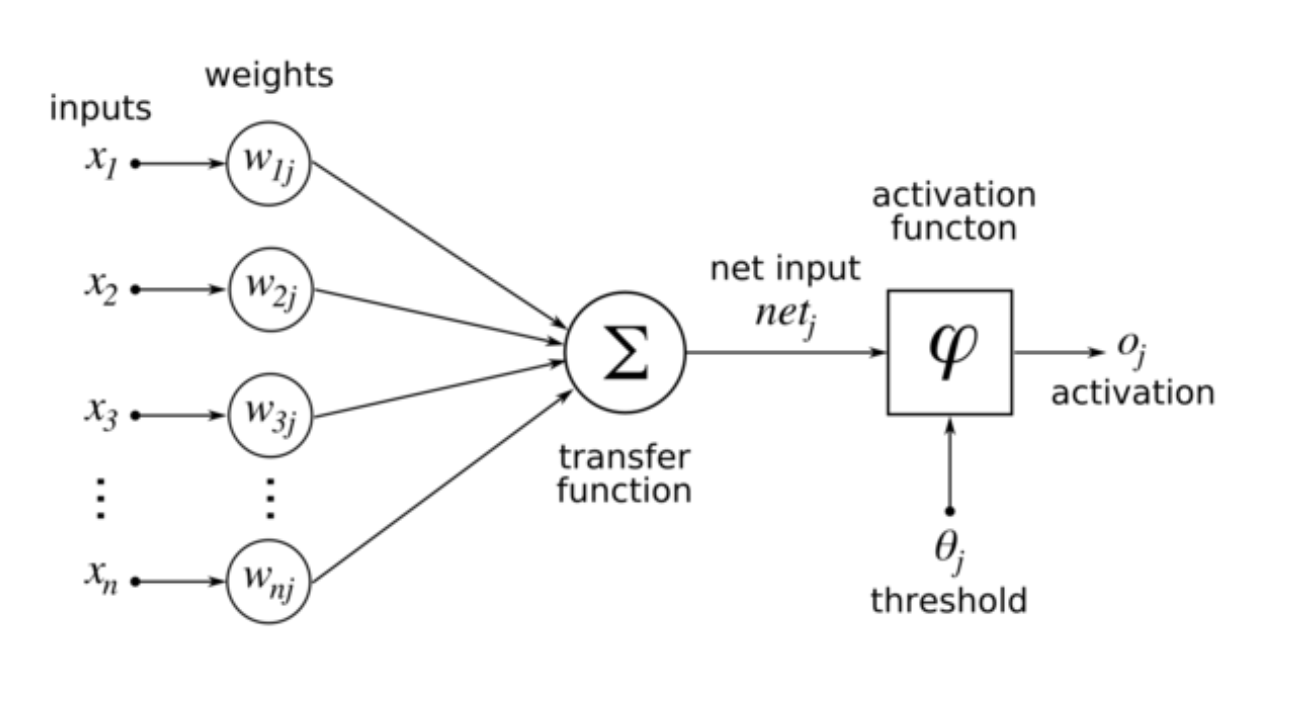
\includegraphics[width=1.00\textwidth]{images/logistic}
\caption{Logistic Regression}
\label{fig:logistic_regression}
\end{figure}

\section{Softmax Regression}
Wie aus der Grafik \ref{fig:softmax_regression} zu entnehmen ist, verfügt die Softmax Regression prinzipiell über einen sehr ähnlichen Aufbau wie die Logistic Regression. Der wesentliche Unterschied zur Logistic Regression liegt jedoch im Output des Models. Im Gegensatz zur Logistic Regression werden die Ausgänge der einzelnen Neuronen nicht in einer Summe an eine Aktivierungsfunktion weitergeleitet, es gibt N Summen der Neuronen, welche in die Softmax Funktionseinheit propagiert werden. Diese entscheidet nun nicht einfach zwischen Ja und Nein, sondern gibt eine Wahrscheinlichkeit für jeden der N möglichen Ausgänge ab, dass es sich um diesen handelt. Dieses Muster eignet sich besonders gut für die Problemstellung der Ziffernerkennung. Sie liefert jeweils für jede Ziffer zwischen 0 und 9 einen Wahrscheinlichkeitswert, der angibt, wie wahrscheinlich es für das Model ist, dass der Input, in diesem Fall ein Bild, eine 0,1,2,…, 9 zeigt. Sucht man jetzt den höchsten Wahrscheinlichkeitswert aus diesem Vektor, erhält man jene Ziffer, von der das Model glaubt, sie auf dem Bild erkannt zu haben.
\begin{figure}[!ht]
\centering
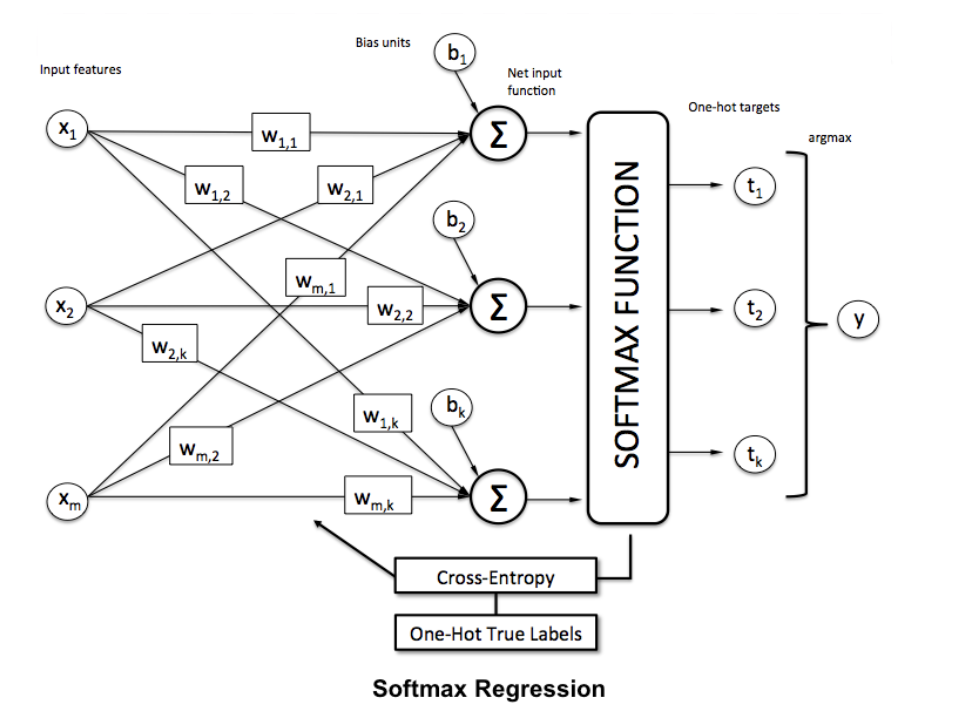
\includegraphics[width=1.00\textwidth]{images/softmax}
\caption{Softmax Regression}
\label{fig:softmax_regression}
\end{figure}

\section{Implementierung}

Um das Model im Python Skript zu implementieren, müssen zuerst einmal die benötigten TensorFlow Variablen und Placeholder angelegt werden.
Der erste Placeholder der gebraucht wird, ist jener der Input-Images. Jedes Bild der MNIST Daten besteht aus 28x28 Pixeln. Reiht man diese Pixel hintereinander, erhält man einen Zeilenvektor der Länge 784. Da die Bilddaten auf diese Weise gespeichert werden sollen, wird mit folgender Zeile ein passender Placeholder angelegt.

\lstset{language=Python}
\definecolor{listinggray}{gray}{0.95} 
\definecolor{keyword}{rgb}{0.4, 0, 0.1} 
\definecolor{comment}{rgb}{0, 0.4, 0}
% Zuweisen der Farben zu den entsprechenden Elementen ... 
\lstset{keywordstyle=\color{keyword}\bfseries} 
\lstset{commentstyle=\color{comment}} 
\lstset{backgroundcolor=\color{listinggray}}

\begin{lstlisting}
x = tf.placeholder(tf.float32, [None, 784], name='InputData')
\end{lstlisting}



Dieser kann eine beliebige Anzahl (None) an Bilddaten (1x784) im Format Float (Grauwerte zwischen 0 und 1) beinhalten und trägt den Namen InputData. Als nächstes wird ein Placeholder gebraucht, der zu jedem Bild das dazugehörige Label abspeichert. Da wir die Labels als One-Hot Vektor geladen haben und 10 mögliche Ausgänge existieren, bildet jedes Label einen Zeilenvektor der Länge 10 ab. Um so einen Placeholder anzulegen, wird folgender Befehl verwendet.

\lstset{language=Python}
\definecolor{listinggray}{gray}{0.95} 
\definecolor{keyword}{rgb}{0.4, 0, 0.1} 
\definecolor{comment}{rgb}{0, 0.4, 0}
% Zuweisen der Farben zu den entsprechenden Elementen ... 
\lstset{keywordstyle=\color{keyword}\bfseries} 
\lstset{commentstyle=\color{comment}} 
\lstset{backgroundcolor=\color{listinggray}}

\begin{lstlisting}
y = tf.placeholder(tf.float32, [None, 10], name = 'LabelData')
\end{lstlisting}

Analog zum InputData Placeholder kann auch dieser eine beliebige Anzahl (None) an Labels (1x10) im Format Float (Wahrscheinlichkeitswert zwischen 0 und 1) beinhalten und trägt den Namen LabelData.
Nachdem nun die Placeholder für den Input angelegt wurden, kann mit den nötigen, modellspezifischen Variablen fortgefahren werden. 
Der Befehl: 


\lstset{language=Python}
\definecolor{listinggray}{gray}{0.95} 
\definecolor{keyword}{rgb}{0.4, 0, 0.1} 
\definecolor{comment}{rgb}{0, 0.4, 0}
% Zuweisen der Farben zu den entsprechenden Elementen ... 
\lstset{keywordstyle=\color{keyword}\bfseries} 
\lstset{commentstyle=\color{comment}} 
\lstset{backgroundcolor=\color{listinggray}}

\begin{lstlisting}
W = tf.Variable(tf.zeros([784, 10]), name='Weights')
\end{lstlisting}

erzeugt eine Variable, welche alle Gewichte zwischen Input und Output beinhaltet. Dies ergibt bei 784 Eingängen und 10 Ausgängen 7840 Gewichte insgesamt. Die letzte benötigte Variable ist jene der Bias-Werte. Für jeden der möglichen Ausgänge wird jeweils ein Wert benötigt, was zu einem Zeilenvektor der Länge 10 führt. Dieser wird folgendermaßen implementiert.


\lstset{language=Python}
\definecolor{listinggray}{gray}{0.95} 
\definecolor{keyword}{rgb}{0.4, 0, 0.1} 
\definecolor{comment}{rgb}{0, 0.4, 0}
% Zuweisen der Farben zu den entsprechenden Elementen ... 
\lstset{keywordstyle=\color{keyword}\bfseries} 
\lstset{commentstyle=\color{comment}} 
\lstset{backgroundcolor=\color{listinggray}}

\begin{lstlisting}
b = tf.Variable(tf.zeros([10]), name = 'Bias')
\end{lstlisting}



Das letzte Stück Code welches benötigt wird, ist jenes des Models an sich.


\lstset{language=Python}
\definecolor{listinggray}{gray}{0.95} 
\definecolor{keyword}{rgb}{0.4, 0, 0.1} 
\definecolor{comment}{rgb}{0, 0.4, 0}
% Zuweisen der Farben zu den entsprechenden Elementen ... 
\lstset{keywordstyle=\color{keyword}\bfseries} 
\lstset{commentstyle=\color{comment}} 
\lstset{backgroundcolor=\color{listinggray}}    
   
\begin{lstlisting}
with tf.name_scope('Model'):
    pred = tf.nn.softmax(tf.matmul(x,W) + b)
\end{lstlisting}
    
    
Die erste Zeile hat prinzipiell keine funktionalen Auswirkungen auf das Model, jedoch hilft es TensorBoard dabei den Graphen übersichtlicher darzustellen, wie man später bemerken wird.
Die zweite Zeile erzeugt nun das eigentliche Model, welches auf Basis der zuvor angelegten Placeholder und Variablen eine Softmax entsprechende Schätzung liefert, um welche Ziffer es sich handelt.





\label{cha:Model}

\chapter{Bewertungsschema}

Nach dem Einbinden der MNIST Daten und dem Erstellen des Models mitsamt allen benötigten Placeholdern und Variablen ist es nun an der Zeit festzustellen, wie nahe die Prädiktionen des Models an der Realität sind. Dafür wird in diesem Workshop eine mathematische Methode namens Cross-Entropy verwendet. In kürzester und einfachster Form beschrieben, liefert Cross-Entropy einen Zahlenwert, welcher die Distanz zwischen dem One-Hot Vektor des Labels mit jenem der Prädiktion liefert. Diese Distanz wird Loss genannt und beschreibt den Fehler des Models bei der Prädiktion. Die Formel von Cross-Entropy lautet dabei: $ - \sum{y' * \ln{y}}$. 

Cross-Entropy
\begin{figure}[!ht]
\centering
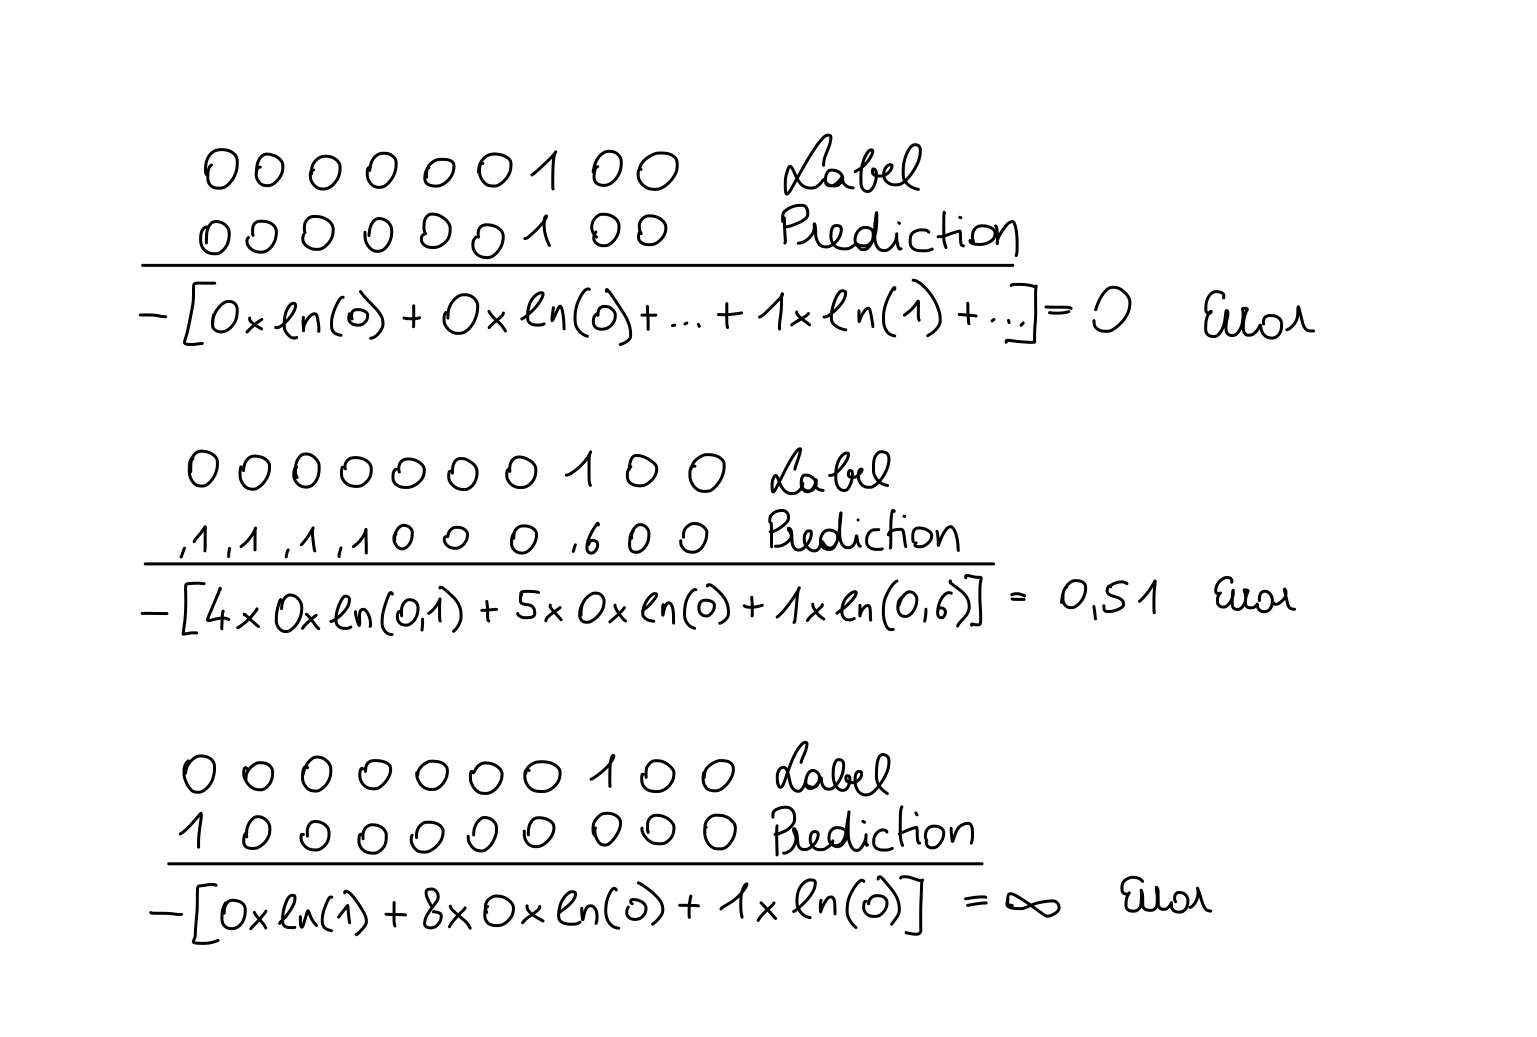
\includegraphics[width=1.00\textwidth]{images/crossEntropy}
\caption{Cross-Entropy Beispiel}
\label{fig:cross_entropy}
\end{figure}

Nun, da ein passendes Bewertungsschema gefunden wurde, ist es an der Zeit, dieses in den Code zu integrieren. Gleich wie beim Model, macht es wiederum Sinn, dieser Funktion einen eigenen \textbf{\textit{name\_scope}} zu geben.

\lstset{language=Python}
\definecolor{listinggray}{gray}{0.95} 
\definecolor{keyword}{rgb}{0.4, 0, 0.1} 
\definecolor{comment}{rgb}{0, 0.4, 0}
% Zuweisen der Farben zu den entsprechenden Elementen ... 
\lstset{keywordstyle=\color{keyword}\bfseries} 
\lstset{commentstyle=\color{comment}} 
\lstset{backgroundcolor=\color{listinggray}}


\begin{lstlisting}
with tf.name_scope('Loss'):
	cost = tf.reduce_mean(-tf.reduce_sum(y*tf.log(pred)))
\end{lstlisting}


	
	
Betrachtet man die zweite Zeile genauer, scheint es eventuell erstmals nicht ganz klar, was hier berechnet wird. Dies ist allerdings schnell geklärt. Der Teil innerhalb von \textbf{\textit{tf.reduce\_mean}} beinhaltet lediglich die mathematische Formel von Cross-Entropy $ - \sum{y' * \ln{y}}$. Da wir allerdings beim Model (pred) möglicherweise nicht nur ein einzelnes Bild evaluieren lassen möchten (die Anzahl der Bilder in InputData ist nicht begrenzt), wird über \textbf{\textit{tf.reduce\_mean}} der Mittelwert über alle Einzelfehler aller zu evaluierenden Bilder berechnet.


\label{cha:Bewertungsschema}
\chapter{Trainieren}

Nachdem nun auch die Möglichkeit der Bewertung des Models gegeben ist, kann damit begonnen werden das Model, basierend auf seinen Fehlern, zu trainieren. Der Ansatz, der in diesem Workshop dazu verwendet wird, lautet Gradient Descent und lässt sich am einfachsten mit einem simplen Beispiel erläutern. Dazu kann man sich einen Bergsteiger vorstellen, der sich auf einem Berggipfel befindet und sich ins Tal begeben will. Dazu kommt, dass der Bergsteiger eine Augenbinde trägt und somit den Weg ins Tal nicht sehen kann. Den Ansatz, den der „Gradient Descent Bergsteiger“ nun wählt, ist folgender:
Zuerst fühlt er mit seinen Füßen den Boden sich selbst herum ab, um das steilste Gefälle rundum ihn zu finden, um daraufhin einen Schritt in diese Richtung zu machen.
Diesen Vorgang wiederholt er so lange, bis der 
\newcounter{zaehler} 
   \begin{list} 
      \usecounter{zaehler} 
       \setcounter{zaehler}{1} 
      \item[\alph{zaehler})]\stepcounter{zaehler} keine Schritte mehr gehen kann. 
      \item[\alph{zaehler})] kein negatives Gefälle mehr fühlen kann und somit annimmt im Tal zu sein.
   \end{list} 


Um dieses Beispiel auf das Training des Models umzumünzen, muss man sich den Berg als Fehlerfunktion des Models (Cross-Entropy), die Position des Bergsteigers als aktuellen Fehler des Models (welcher sich durch das aktuelle Weight-Setup ergibt) und den Schritt des Bergsteigers den Berg hinab als Lernschritt beim trainieren des Models vorstellen. Zwei wichtige Parameter beim Training sind dabei zum einen die initialen Gewichte des Models und zum anderen die Learning-Rate.


\section{Initiale Gewichte}
Die initialen Gewichte des Models spiegeln dabei die Startposition des Bergsteigers auf seinem Weg ins Tal wieder. Wählt man die initialen Gewichte geschickt aus, beginnt die Reise des Bergsteigers relativ nahe über dem Tal, werden sie ungeschickt gewählt, muss der Bergsteiger seinen Abstieg am Gipfel des Berges, am maximalen Fehler, beginnen. 


\section{Learning Rate}
Die Learning-Rate gibt an, wie viel das Model auf einmal lernen kann. Dies ist wiederum vorstellbar mit der Schrittlänge, die der Bergsteiger hat. Wird die Learning-Rate zu groß gewählt, kann es dazu kommen, dass der Fehler nicht wie erwünscht immer kleiner wird mit jeder Iteration, sondern dass sich dieser mit jeder Iteration immer weiter aufschaukelt.
Wird sie allerdings zu klein gewählt, sind die Lernschritte äußerst klein und der Lernvorgang dauert somit sehr lange und benötigt eine enorme Menge an Trainingsdaten.

\section{Implementierung}

Um das Modell zu trainieren müssen folgende Zeilen Code hinzugefügt werden. Zunächst müssen drei Parameter definiert werden:

\lstset{language=Python}
\definecolor{listinggray}{gray}{0.95} 
\definecolor{keyword}{rgb}{0.4, 0, 0.1} 
\definecolor{comment}{rgb}{0, 0.4, 0}
% Zuweisen der Farben zu den entsprechenden Elementen ... 
\lstset{keywordstyle=\color{keyword}\bfseries} 
\lstset{commentstyle=\color{comment}} 
\lstset{backgroundcolor=\color{listinggray}}

\begin{lstlisting}
learning_rate = 0.01 
#Gibt an wie schnell gelernt werden kann.

training_epochs = 30
#Gibt an wie oft das Model trainiert werden soll. Vergleichbar mit der Anzahl der Schritte die der Bergsteiger gehen darf.

batch_size = 100
#In jeder Epoche wird das Model mit allen MNIST Trainings-Datensätzen trainiert. Die Batch Size gibt dabei an wie groß die einzelnen Chargen an Datensätzen sein sollen.

\end{lstlisting}

Als nächstes muss wiederum eine Funktion angelegt werden, die den eigentlichen Lernvorgang, in diesem Fall mit Hilfe von Gradient Descent, abbildet:

\lstset{language=Python}
\definecolor{listinggray}{gray}{0.95} 
\definecolor{keyword}{rgb}{0.4, 0, 0.1} 
\definecolor{comment}{rgb}{0, 0.4, 0}
% Zuweisen der Farben zu den entsprechenden Elementen ... 
\lstset{keywordstyle=\color{keyword}\bfseries} 
\lstset{commentstyle=\color{comment}} 
\lstset{backgroundcolor=\color{listinggray}}

\begin{lstlisting}
with tf.name_scope('Optimizer'):
    optimizer = tf.train.GradientDescentOptimizer(learning_rate).minimize(cost)
\end{lstlisting}


Wiederum in einem eigenen \textbf{\textit{name\_scope}} wird hier ein Gradient Descent Optimizer erstellt, der mit der vorhin definierten Learning-Rate versucht, die Kosten-cost (Cross-Entropy)-zu minimieren. Nun kann begonnen werden das Model zu trainieren, dazu müssen zuerst alle TensorFlow Variablen initialisiert werden. Dies geschieht mit dem Befehl.

\lstset{language=Python}
\definecolor{listinggray}{gray}{0.95} 
\definecolor{keyword}{rgb}{0.4, 0, 0.1} 
\definecolor{comment}{rgb}{0, 0.4, 0}
% Zuweisen der Farben zu den entsprechenden Elementen ... 
\lstset{keywordstyle=\color{keyword}\bfseries} 
\lstset{commentstyle=\color{comment}} 
\lstset{backgroundcolor=\color{listinggray}}

\begin{lstlisting}
init = tf.global_variables_initializer()
\end{lstlisting}


Im nächsten Schritt wird eine TensorFlow Session eröffnet, mit deren Hilfe erst die einzelnen Funktionen ausgeführt werden können.


\lstset{language=Python}
\definecolor{listinggray}{gray}{0.95} 
\definecolor{keyword}{rgb}{0.4, 0, 0.1} 
\definecolor{comment}{rgb}{0, 0.4, 0}
% Zuweisen der Farben zu den entsprechenden Elementen ... 
\lstset{keywordstyle=\color{keyword}\bfseries} 
\lstset{commentstyle=\color{comment}} 
\lstset{backgroundcolor=\color{listinggray}}

\begin{lstlisting}
with tf.Session() as sess:
    sess.run(init)
    #training
    for epoch in range(training_epochs):
        avg_cost = 0.0
        total_batch = int(mnist.train.num_examples/batch_size)
        #loop over all batches
        for i in range(total_batch):
            batch_xs, batch_ys = mnist.train.next_batch(batch_size)
            opt, c = sess.run([optimizer, cost], feed_dict={x: batch_xs, y: batch_ys})
            avg_cost += c / total_batch

        if (epoch+1) % 1 == 0:
            print(avg_cost)

\end{lstlisting}

Dieser Code initialisiert zuerst alle Variablen und fährt dann fort mit dem eigentlichen Training. Dazu wird \textbf{\textit{training\_epochs}} mal das gesamte Trainingsdaten-Set vom MNIST in \textbf{\textit{batch\_size}} große Stücke zerlegt und jeweils nacheinander in die Placeholder InputData und LabelData geladen. Daraufhin wird auf Basis der Daten in den Placeholdern sowohl der Fehler des Models berechnet (cost), als auch der Optimizer gestartet, welcher das Model iterativ verbessert. Darüber hinaus wird aus Visualisierungsgründen der durchschnittliche Fehler berechnet und auf der Konsole ausgegeben. Durch die Ausgabe auf der Konsole kann über jede Epoche hinweg mitverfolgt werden, wie der Fehler stetig kleiner wird.




\label{cha:Trainieren}
\chapter{Evaluieren und Visualisieren}

\section{Accuracy}
Fertig! Die eigentliche Arbeit ist somit erledigt und das Model wurde trainiert. Nun möchte man möglicherweise evaluieren, wie gut das Model performt. Dies kann relativ einfach durch das Hinzufügen einer weiteren Funktion erledigt werden.

\lstset{language=Python}
\definecolor{listinggray}{gray}{0.95} 
\definecolor{keyword}{rgb}{0.4, 0, 0.1} 
\definecolor{comment}{rgb}{0, 0.4, 0}
% Zuweisen der Farben zu den entsprechenden Elementen ... 
\lstset{keywordstyle=\color{keyword}\bfseries} 
\lstset{commentstyle=\color{comment}} 
\lstset{backgroundcolor=\color{listinggray}}

\begin{lstlisting}
with tf.name_scope('Accuracy'):
    acc = tf.equal(tf.argmax(pred,1), tf.argmax(y, 1))
    acc = tf.reduce_mean(tf.cast(acc, tf.float32))
\end{lstlisting}


Die Accuracy vergleicht dabei das Ergebnis des Models mit dem Label des Datensatzes und notiert sich eine 1, wenn diese übereinstimmen und eine 0, wenn nicht. Im nächsten Schritt wird ein Mittelwert über alle Prädiktionen gebildet, was einen Wert ergibt, der eine prozentuelle Übereinstimmung zwischen Prädiktion und Label widerspiegelt. Um diesen Wert in der Konsole anzeigen zu lassen, muss einfach folgender Befehl an das Ende des Session Bereichs hinzugefügt werden:

\lstset{language=Python}
\definecolor{listinggray}{gray}{0.95} 
\definecolor{keyword}{rgb}{0.4, 0, 0.1} 
\definecolor{comment}{rgb}{0, 0.4, 0}
% Zuweisen der Farben zu den entsprechenden Elementen ... 
\lstset{keywordstyle=\color{keyword}\bfseries} 
\lstset{commentstyle=\color{comment}} 
\lstset{backgroundcolor=\color{listinggray}}

\begin{lstlisting}
print("Accuracy: ", acc.eval({x: mnist.test.images, y: mnist.test.labels}))
\end{lstlisting}

Will man außerdem visuell Einsicht in die geleistete Arbeit werfen, eignet sich TensorBoard perfekt dafür. In diesem Workshop werden folgende Visualisierungen mit Hilfe von TensorBoard implementiert:



\section{Graph}

Will man sich den Graphen, welcher den Datenfluss dieses Scripts zeigt, anzeigen lassen, sind folgende Codeteile einzufügen:

\lstset{language=Python}
\definecolor{listinggray}{gray}{0.95} 
\definecolor{keyword}{rgb}{0.4, 0, 0.1} 
\definecolor{comment}{rgb}{0, 0.4, 0}
% Zuweisen der Farben zu den entsprechenden Elementen ... 
\lstset{keywordstyle=\color{keyword}\bfseries} 
\lstset{commentstyle=\color{comment}} 
\lstset{backgroundcolor=\color{listinggray}}

\begin{lstlisting}
logs_path = 'tf_logs'
\end{lstlisting}


Diese Zeile muss zu den anderen Parametern am Anfang des Scripts hinzugefügt werden und gibt an, in welches Verzeichnis TensorFlow die serialisierten Graph-Daten für TensorBoard speichern soll.

Danach muss am Beginn des Session Bereichs im Script folgende Zeile eingefügt werden um einen FileWriter zu erzeugen, welcher den Graphen serialisiert und an den definierten Pfad (\textbf{\textit{logs\_path}}) speichert:

\lstset{language=Python}
\definecolor{listinggray}{gray}{0.95} 
\definecolor{keyword}{rgb}{0.4, 0, 0.1} 
\definecolor{comment}{rgb}{0, 0.4, 0}
% Zuweisen der Farben zu den entsprechenden Elementen ... 
\lstset{keywordstyle=\color{keyword}\bfseries} 
\lstset{commentstyle=\color{comment}} 
\lstset{backgroundcolor=\color{listinggray}}

\begin{lstlisting}
summary_writer = tf.summary.FileWriter(logs_path, graph= tf.get_default_graph()) 
\end{lstlisting}


Am Ende des Session Bereichs im Script muss zusätzlich folgendes Statement eingefügt werden, um den FileWriter wieder ordnungsgemäß zu schließen:

\lstset{language=Python}
\definecolor{listinggray}{gray}{0.95} 
\definecolor{keyword}{rgb}{0.4, 0, 0.1} 
\definecolor{comment}{rgb}{0, 0.4, 0}
% Zuweisen der Farben zu den entsprechenden Elementen ... 
\lstset{keywordstyle=\color{keyword}\bfseries} 
\lstset{commentstyle=\color{comment}} 
\lstset{backgroundcolor=\color{listinggray}}

\begin{lstlisting}
summary_writer.close()
\end{lstlisting}


Wird nun das Script ausgeführt und TensorBoard gestartet, kann unter dem Tab \textbf{„Graph“} der Graph eingesehen werden.

\section{Skalare}

Eine weitere Möglichkeit TensorBoard sinnvoll einzusetzen ist, bestimmte Skalare zu definieren, die im Laufe des Trainings geloggt werden, um deren Verlauf in TensorBoard nachvollziehbar zu machen. In diesem Fall werden Skalare für den Fehler und die Accuracy gebildet:

\lstset{language=Python}
\definecolor{listinggray}{gray}{0.95} 
\definecolor{keyword}{rgb}{0.4, 0, 0.1} 
\definecolor{comment}{rgb}{0, 0.4, 0}
% Zuweisen der Farben zu den entsprechenden Elementen ... 
\lstset{keywordstyle=\color{keyword}\bfseries} 
\lstset{commentstyle=\color{comment}} 
\lstset{backgroundcolor=\color{listinggray}}

\begin{lstlisting}
tf.summary.scalar("loss", cost)
tf.summary.scalar("accuracy", acc)
merged_summary_op = tf.summary.merge_all()
\end{lstlisting}


Dieser Code muss vor dem Beginn des Session Bereichs implementiert werden und erstellt jeweils einen Skalar für den Fehler und die Accuracy. Der dritte Befehl wird benötigt, damit alle Summaries im Graph verwendet werden. Um nun diese Skalare zu loggen, muss folgende Zeile im Session Bereich:

\lstset{language=Python}
\definecolor{listinggray}{gray}{0.95} 
\definecolor{keyword}{rgb}{0.4, 0, 0.1} 
\definecolor{comment}{rgb}{0, 0.4, 0}
% Zuweisen der Farben zu den entsprechenden Elementen ... 
\lstset{keywordstyle=\color{keyword}\bfseries} 
\lstset{commentstyle=\color{comment}} 
\lstset{backgroundcolor=\color{listinggray}}

\begin{lstlisting}
opt, c = sess.run([optimizer, cost], feed_dict={x: batch_xs, y: batch_ys})
\end{lstlisting}

durch diese ersetzt werden: 

\lstset{language=Python}
\definecolor{listinggray}{gray}{0.95} 
\definecolor{keyword}{rgb}{0.4, 0, 0.1} 
\definecolor{comment}{rgb}{0, 0.4, 0}
% Zuweisen der Farben zu den entsprechenden Elementen ... 
\lstset{keywordstyle=\color{keyword}\bfseries} 
\lstset{commentstyle=\color{comment}} 
\lstset{backgroundcolor=\color{listinggray}}

\begin{lstlisting}
opt, c, summary = sess.run([optimizer, cost, merged_summary_op], feed_dict={x: batch_xs, y: batch_ys})
\end{lstlisting}

und darüber hinaus jene Zeile gleich danach eingefügt werden:             

\lstset{language=Python}
\definecolor{listinggray}{gray}{0.95} 
\definecolor{keyword}{rgb}{0.4, 0, 0.1} 
\definecolor{comment}{rgb}{0, 0.4, 0}
% Zuweisen der Farben zu den entsprechenden Elementen ... 
\lstset{keywordstyle=\color{keyword}\bfseries} 
\lstset{commentstyle=\color{comment}} 
\lstset{backgroundcolor=\color{listinggray}}

\begin{lstlisting}
summary_writer.add_summary(summary, epoch*total_batch + i)
\end{lstlisting}


Analog zum Graph muss auch hier das Script und TensorBoard ausgeführt werden, um den Trace der beiden Skalare über den Trainingsprozess hinweg nachverfolgen zu können.

\section{Projektor}

Der Projektor bietet die Möglichkeit, die 784 Dimensionen eines MNIST Bildes auf 3 Dimensionen zu reduzieren und somit die einzelnen Bilder der MNIST Datenbank im Dreidimensionalen Raum gegenüberzustellen. Dazu müssen im Code zweierlei Daten zu Verfügung gestellt werden: Metadaten und Embeddings. Metadaten werden dazu benötigt, den Bezug eines Bildes zum entsprechenden Label herstellen zu können. Dies kann gemacht werden, indem man mit folgendem Code eine Datei erstellt, die Zeilenweise die Labels, jedoch nicht im One-Hot Format, zu jedem Bild der Trainingsdaten enthält.

\lstset{language=Python}
\definecolor{listinggray}{gray}{0.95} 
\definecolor{keyword}{rgb}{0.4, 0, 0.1} 
\definecolor{comment}{rgb}{0, 0.4, 0}
% Zuweisen der Farben zu den entsprechenden Elementen ... 
\lstset{keywordstyle=\color{keyword}\bfseries} 
\lstset{commentstyle=\color{comment}} 
\lstset{backgroundcolor=\color{listinggray}}

\begin{lstlisting}
metadata = os.path.join(logs_path, 'metadata.tsv')
with open(metadata, 'w') as metadata_file:
    for row in mnistTwo.test.labels:
        metadata_file.write('%d\n' % row)
\end{lstlisting}

Die Postion dieses Codestücks liegt wiederum vor dem Session Bereich. Innerhalb des Session Bereichs werden nun die Embeddings konfiguriert:

\lstset{language=Python}
\definecolor{listinggray}{gray}{0.95} 
\definecolor{keyword}{rgb}{0.4, 0, 0.1} 
\definecolor{comment}{rgb}{0, 0.4, 0}
% Zuweisen der Farben zu den entsprechenden Elementen ... 
\lstset{keywordstyle=\color{keyword}\bfseries} 
\lstset{commentstyle=\color{comment}} 
\lstset{backgroundcolor=\color{listinggray}}

\begin{lstlisting}
saver = tf.train.Saver([images])
saver.save(sess, os.path.join(logs_path, 'images.ckpt'))
config = projector.ProjectorConfig()
    embedding = config.embeddings.add()
    embedding.tensor_name = images.name
    embedding.sprite.image_path = os.path.join(logs_path, 'sprite.png')
    embedding.metadata_path = metadata
    embedding.sprite.single_image_dim.extend([28,28])

    projector.visualize_embeddings(tf.summary.FileWriter(logs_path), config)
\end{lstlisting}



Hier werden sowohl die vorhin erstellten Metadaten zu den Embeddings hinzugefügt, als auch ein Sprite Image angegeben, welches die einzelnen Bilder der MNIST Daten als Thumbnails in einem .png File vereint. Zum Schluss noch das Visualisieren der Embeddings laut den gerade erstellten Settings (Sprite Image, Metadata) aktiviert. Durch Ausführen des Scripts und das Aktivieren von TensorBoard kann nun im Tab Projektor und unter T-SNE als Dimensions-Reduktions Algorithmus die dimensionale Trennung der einzelnen Datensätze begutachtet werden.

Diese Ansicht ist analog zu jener einfachen Klassifizierung zu sehen, nur dass es sich bei MNIST Bildern nicht um 2 sondern um 784 auf 3 Dimensionen reduzierte Daten handelt.


\label{cha:Evaluieren und Visualisieren}
\chapter{Closing Remarks}
\label{cha:Closing}


%%%----------------------------------------------------------
\appendix                                         % appendix 
%%%----------------------------------------------------------

%\chapter{Technical Details}
\label{app:TechnicalDetails}



	% technical supplements
%\chapter{CD-ROM/DVD Contents}
\label{app:cdrom}


	% contents of the CD-ROM/DVD
%\chapter{Questionnaire}
\label{app:Questionnaire}





	% chronological list of changes
%\chapter{\latex Source Code}
\label{app:SourceCode}

	% source text of this document

%%%----------------------------------------------------------
\MakeBibliography                        				% references
%%%----------------------------------------------------------

%%% special page for checking print size --------------------
\chapter*{Check Final Print Size}

\begin{center}
{\Large --- Check final print size! ---}

\bigskip

\calibrationbox{100}{50} % width/height of box in mm

\bigskip

{\Large --- Remove this page after printing! ---}

\end{center}



%%%----------------------------------------------------------
\end{document}
%%%----------------------------------------------------------